\documentclass[12pt]{article}
% Эта строка — комментарий, она не будет показана в выходном файле
\usepackage{ucs}
\usepackage[utf8x]{inputenc} % Включаем поддержку UTF8
\usepackage[russian]{babel}  % Включаем пакет для поддержки русского языка
\usepackage{amsmath}
\usepackage{mathtools}
\usepackage{amssymb}
% \usepackage[dvips]{graphicx}
% \graphicspath{{noiseimages/}}
\usepackage[pdftex]{graphicx}


% Параметры страницы: 1см от правого края и 2см от остальных.


\hoffset=0mm
\voffset=0mm
\textwidth=180mm        % ширина текста
\oddsidemargin=-6.5mm   % левое поле 25.4 - 5.4 = 20 мм
\textheight=240mm       % высота текста 297 (A4) - 40
\topmargin=-15.4mm      % верхнее поле (10мм)
\headheight=5mm      % место для колонтитула
\headsep=5mm          % отступ после колонтитула
\footskip=8mm         % отступ до нижнего колонтитула
% \setlength{\textheight}{263mm}
\begin{document}
    \author {Зотов Алексей 496 гр.}
    \title {Лабораторная работа 1.2 \\ Определение моментов инерции твердых тел с помощью трифилярного подвеса}
    \maketitle{}   
    
    \indent
    \textbf{Цель работы:} измерение момента инерции ряда тел и сравнение результатов с расчетами по теоретическим формулам; проверка аддттивности моментов инерции и справедливости формулы Гюйгенса– Штейнера.
    \\\newline
    \indent
    \textbf{В работе используются:} трифилярный подвес, секундомер, счетчик числа колебаний, набор тел, момент инерции которых надлежит измерить (диск, стержень, полый цилиндр и другие).
    \\\newline
    
    \textbf{Определение.} Моментом инерции твердого тела (или системы тел) относительно выбранной оси, называется величина, определяемая соотношением: 
    \begin{equation}
              I = \int r^2dm
    \end{equation} 
    
    Из определения момента инерции и по 2-му закону Ньютона для движения материальной точки под действием силы $\vec{F}$, учитывая $v = \omega r$ , уравнение вращательного движения принимает вид:

    \begin{equation}
              I \frac{d\omega}{dt} = M \quad \text{где $M$ - момент силы $\vec{F}$}
    \end{equation} 

    \textbf{Теорема Гюйгенса–Штейнера.} Момент инерции $I$ относительно произвольной оси равен сумме момента инерции $I_0$ относительно оси, параллельной ей и проходящей через центр масс тела, и произведения массы тела $m$ на квадрат расстояния между осями $a_0$:
    \begin{equation}
        I = I_0 + ma^2_0
    \end{equation} \\\newline

    \textbf{Экспериментальная установка.} Будем использовать устройство, показанное на рис. 1 и называемое трифилярным подвесом. Оно состоит из укрепленной на некоторой высоте неподвижной платформы $P$ и подвешенной к ней на трех симметрично расположенных нитях $AA'$, $BB'$ и $CC'$ вращающейся платформы $P'$.

    Платформа $P$ укреплена на кронштейне и снабжена рычагом (на рисунке не показан), при помощи которого в системе создадим крутильные колебания путем небольшого поворота верхней платформы.

    Для счета числа колебаний используется счетчик, состоящий из осветителя (2), фотоэлемента (3) и пересчетного устройства (1). Легкий лепесток, укрепленный на платформе, при колебаниях пересекает световой луч дважды за период. Соответствующие сигналы от фотоэлемента поступают на пересчетное устройство.

    \begin{center} 
        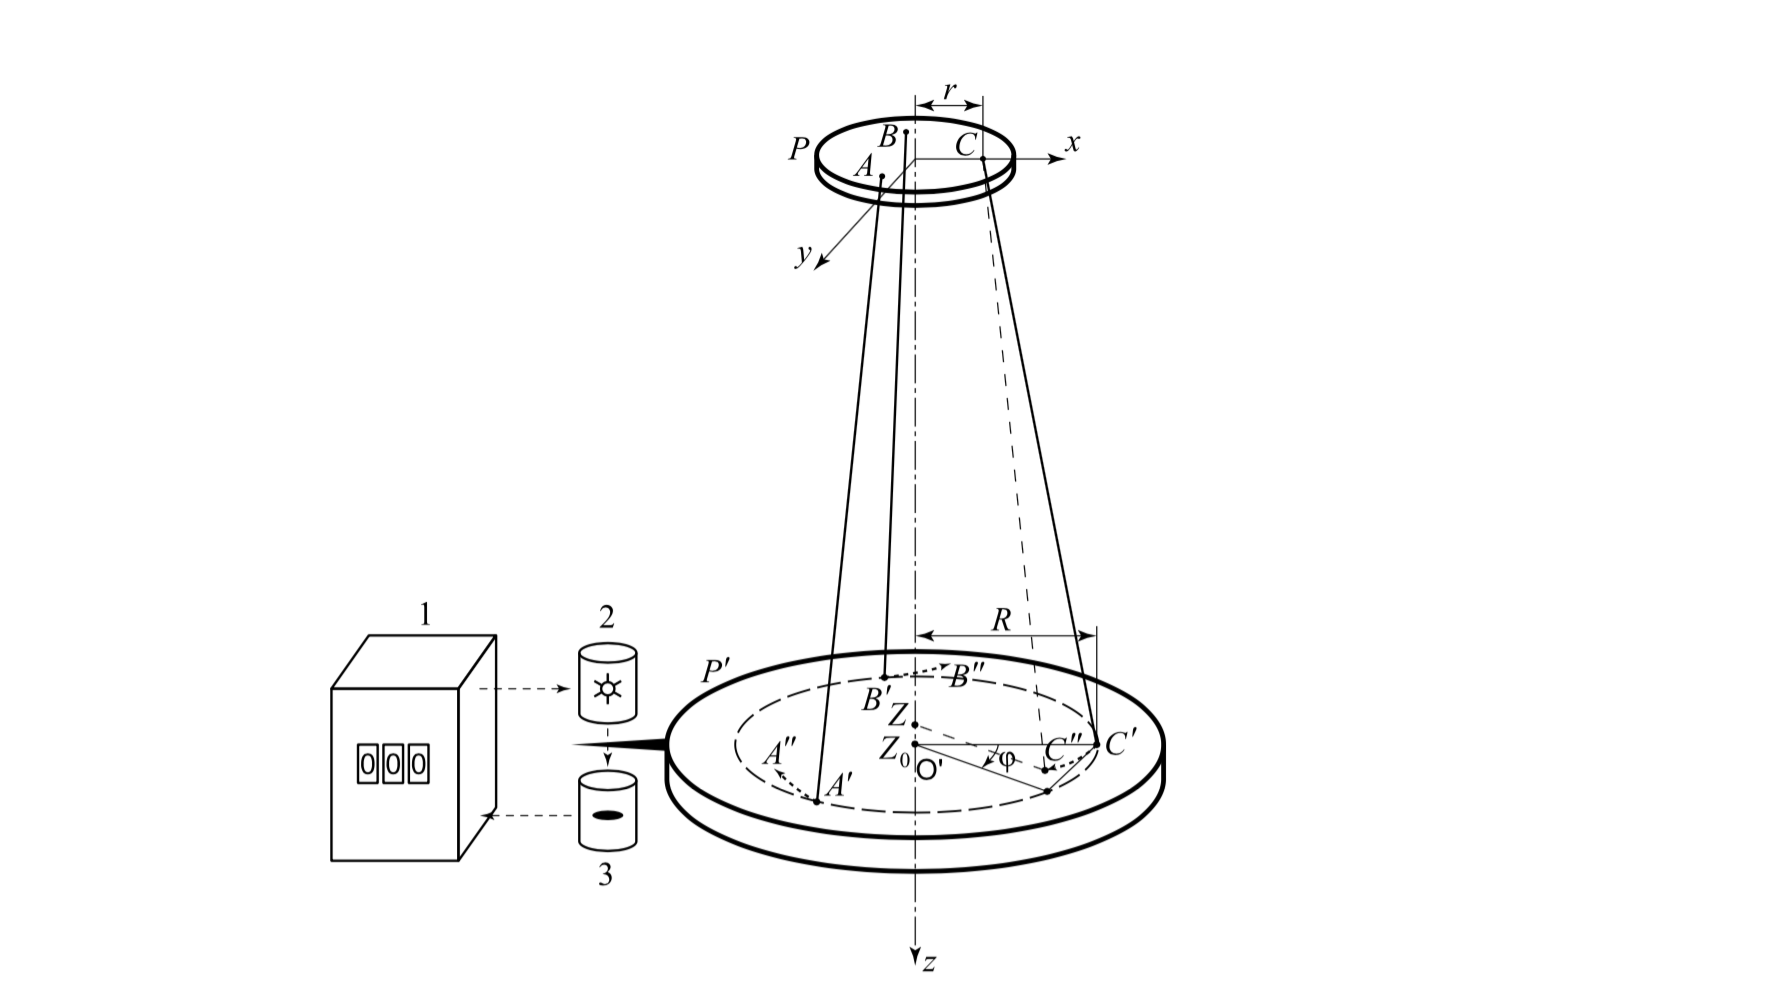
\includegraphics[width=5in]{trif2.png} \\ Рис. 1: трифилярный подвес
    \end{center}
    
    \textbf{Уравнение гармонических колебаний.} Уравнение малых колебаний трифилярного подвеса выглядит следующим образом:
    \begin{equation}
        I\ddot{\varphi} + mg \frac{Rr}{z_0}\varphi = 0
    \end{equation} 
    где $I$ — момент инерции тела вместе с платформой, $m$ — их суммарная масса, $z_0$ — расстояние от центра нижней платформы $O'$ до центра верхней $O$ в положении равновесия, а $R$ и $r$ — расстояния от оси вращения до точки крепления нити на нижней и на верхней платформах соответственно (см. рис. 2).

    Решение уравнения (4) представляет собой гармонические колебания:
    \begin{equation}
        \varphi(t) = \varphi_m \sin(2\pi t/T + \theta)
    \end{equation} 
    где амплитуда $\varphi_m$ и фаза $\theta$ определяются начальными условиями, а
    {\itshapeпериод колебаний} равен
    \begin{equation}
        T = 2 \pi \sqrt{\frac{I z_0}{mgRr}}
    \end{equation} 
    положим $k = \frac{gRr}{4\pi^2z_0}$ , эта величина постоянна для данной установки. Тогда момент инерции можно выразить следующим образом:
    \begin{equation}
        I = kmT^2
    \end{equation}

    Таким образом, полученные формулы позволяют определить момент
    инерции платформы с телом и отдельно платформы по соответствующим периодам крутильных колебаний.

    \textbf{Аддитивность моментов инерции.} Момент инерции самого тела можно вычислить, воспользовавшись аддитивностью $I_{A+B}$ — момент инерции составного тела (A+B) равен сумме моментов инерции его частей A и B :
        \begin{equation}
            I_{A+B} = I_A + I_B
        \end{equation} 
    \\ \\ \\ 
    \textbf{\large Ход работы}
    \begin{enumerate} 
        \item \underline{Параметры установки.} \\\newline
            $R_0 = (114.6 \pm 0.5)mm.$ \\ $r_0 = (30.2 \pm 0.3)mm. \\
            m_0 = (448.2 \pm 0.3)g.$ \\ $z_0 = (214 \pm 1)cm.$\\ \\
            $\Delta k = \frac{g}{4\pi^2} \sqrt{(\frac{r_0 \Delta R_0}{z_0})^2 + (\frac{R_0 \Delta r_0}{z_0})^2 
            + (\frac{r_0R_0 \Delta z_0}{z_0^2})^2}$ \\
            $ k = (3.9920 \pm 0.0699)* 10 ^ {-4} \quad [m^2 / c^2]$ \\ \\
            $I_0 = (\frac{R_0^2 M_0}{2} = (2.9431 \pm 0.0154) * 10 ^{-3}) \quad [m^2 * kg]$

        \item \underline{Пустая платформа, определение погрешности.} \\ \\
            Измерим период колебаний пустой платформы: \\
            $N_T = 20$ - количество полных колебаний на 1 измерение. \\
            $n = 6$ - количество измерений. 
            
            \begin{table}[ht]
                \caption{Измерения вермени 40 колебаний пустой платформы.}
                \begin{center}
                \begin{tabular}{|c|c|c|c|c|c|c|}
                \hline 
                $i$ & 1 & 2 & 3 & 4 & 5 & 6 \\
                \hline
                $t_i$,c & 86.546 & 86.435 & 86.614 & 87.299 & 87.325 & 87.148 \\
                \hline
                \end{tabular}
                \end{center}
            \end{table}

            среднее время 20 колебаний: $t_{cp} = 86.8945$(c) \\ \\
            среднее время одного колебания: $T_{cp} = \frac{t_{cp}}{20} = 4.344725 \approx 4.345$(c) \\ \\ 
            погрешность измерения: $\sigma = \sqrt{\frac{\Sigma (t_i - t_{cp})^2 }{n-1}} \approx 0.3957$ \\ \\
            относительная погрешность измеряемой величины: $\varepsilon = \frac{\sigma}{N* T_{cp}}$ \\ 
            положим $N = 19 \implies \varepsilon < 0.0048 < 0.005$ \\ 
        \item \underline{Измерения с различными телами}
            \begin{enumerate} 
                \item \underline{Диск} \\
                    $R = (8.5 \pm 0.025)cm$  - радиус диска \\ 
                    % $r = (0.5 \pm 0.025)cm$ - радиус выступа \\
                    % $h = (2.4 \pm 0.025)cm$ - высота выступа  \\
                    $m = 580.1 g$ - общая масса\\ \\
                    $t = 69.189 \implies T \approx 3.5047$(с) - измеренный период \\
                     
                    $I_1 = k(m + m_0)T^2 - I_0 = (2.0976 \pm 0.0658) * 10 ^ {-3} \quad [m^2 * kg]$ - измеренный момент \\
                    $I_2 = R^2 * m/ 2 = 2.0956 * 10^{-3}$ - теоретический результат, с учетом погрешности совпадает с результатом, полученным из опыта.
                    

                \item \underline{Кольцо} \\
                    $R = (8.4 \pm 0.025)cm$  - радиус кольца \\ 
                    $d = (0.5 \pm 0.025)cm$ - толщина стенки кольца  \\
                    $m = 975.2 g$ - общая масса\\ \\
                    $t = 79.027(c) \implies T \approx 4.16(с)$ \\ \\ 
                    $I_1 = (6.8905 \pm 0.0984) * 10^{-3} \quad [m^2 * kg]$ - измеренный момент
                    $I_2 = 6.8810 * 10 ^ {-3}$ - теоретический результат, с учетом погрешности, совпадает с результатом, полученным из опыта.

                \item \underline{Брус} \\
                    $M = 706.5 g$ - общая масса\\ 
                    $l = (21 \pm 0.05)cm$ - длина  \\
                    $d_{cp} = (2 \pm 0.025)cm$ - толщина\\ \\
                    \begin{table}[h]
                        \caption{Измерения толщины бруса.}
                        \begin{center}
                        \begin{tabular}{|c|c|c|c|c|c|}
                            \hline 
                                $i$ & 1 & 2 & 3 & 4 & 5 \\
                            \hline
                                $d_i,cm$ & 2.0 & 2.0 & 2.0 & 2.0 & 2.0 \\
                            \hline
                        \end{tabular}
                        \end{center}
                    \end{table}
                    
                    $t = 68.840(c) \implies T \approx 3.623(c)$ \\ 
                    $I_1 = (3.1084 \pm 0.0605) * 10^{-3} \quad [m^2 * kg]$ \\
                    $I_2 = 2.596 * 10 ^ {-3}$
                \item \underline{Диск + Кольцо} \\
                    $t = 72.837(c) \implies T \approx 3.834(c)$

                    $I = (8.8137 \pm 0.117582) * 10^{-3} \quad [m^2 * kg]$ \\
                    По закону аддитивности $I = I_d + I_k = (8.9881 \pm 0.16416) * 10^{-3}$, что, с учетом погрешности, удовлетворяет результатам опыта.
                \item \underline{Полудиск} \\
                    $M = 566.4g$ \\ 
                    $R = (4.15 \pm 0.025)cm$ \\ \\
                    Расположим диски как показано на рисунке 2. Найдем зависимость $T(h)$ периода колебаний от расстояния до центра платформы.
                    \begin{center} 
                        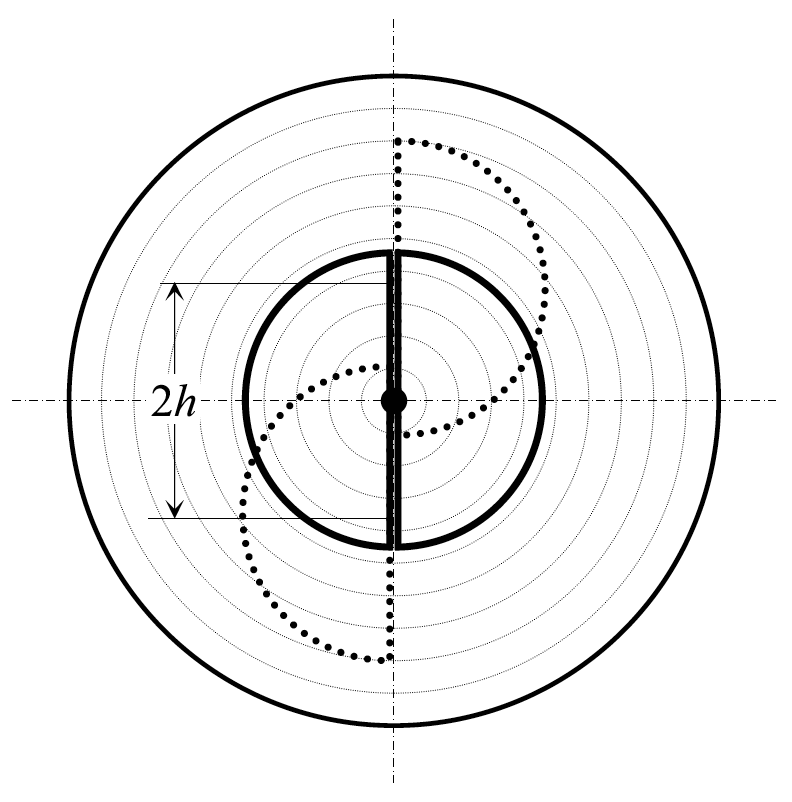
\includegraphics[width=2.5in]{disk.png} \\ Рис. 2: расположение дисков на платформе.
                    \end{center}

                    \begin{table}[h]
                        \caption{Период колебаний и расположение дисков.}
                        \begin{center}
                        \begin{tabular}{|c|c|c|c|c|c|c|c|c|c|}
                            \hline 
                                $h$ & 0 & 0.45 & 1.375 & 2.85 & 3.35 & 4.35 & 5.35 & 7.35 \\
                            \hline
                                $t,c$ & 50.532 & 50.686 & 52.048 & 55.297 & 57.383& 61.748 & 66.124 & 76.614 \\
                            \hline
                                $T,c$ & 2.6596 & 2.6677 & 2.7394 & 2.9104 & 3.0202 & 3.2499 
                                & 3.4802 & 4.0323 \\
                            \hline
                        \end{tabular}
                        \end{center}
                    \end{table}


                    \begin{table}[h]
                        \caption{Данные для построения графика $I(h^2)$}
                        \begin{center}
                        \begin{tabular}{|c|c|c|c|c|c|c|c|c|c|}
                            \hline 
                                $h , [m]$ & 0.0 & 2e-05 & 0.00019 & 0.00081 & 0.00112 & 0.00189 & 0.00286 & 0.0054 \\
                            \hline
                                $I(h^2) , [kg * m^2]$ & 0.00152 & 0.00155 & 0.00179 & 0.0024 & 0.00281 & 0.00372 & 0.0047 & 0.00732 \\
                            \hline
                            \end{tabular}
                        \end{center}
                    \end{table}
            \end{enumerate}
            \begin{center} 
                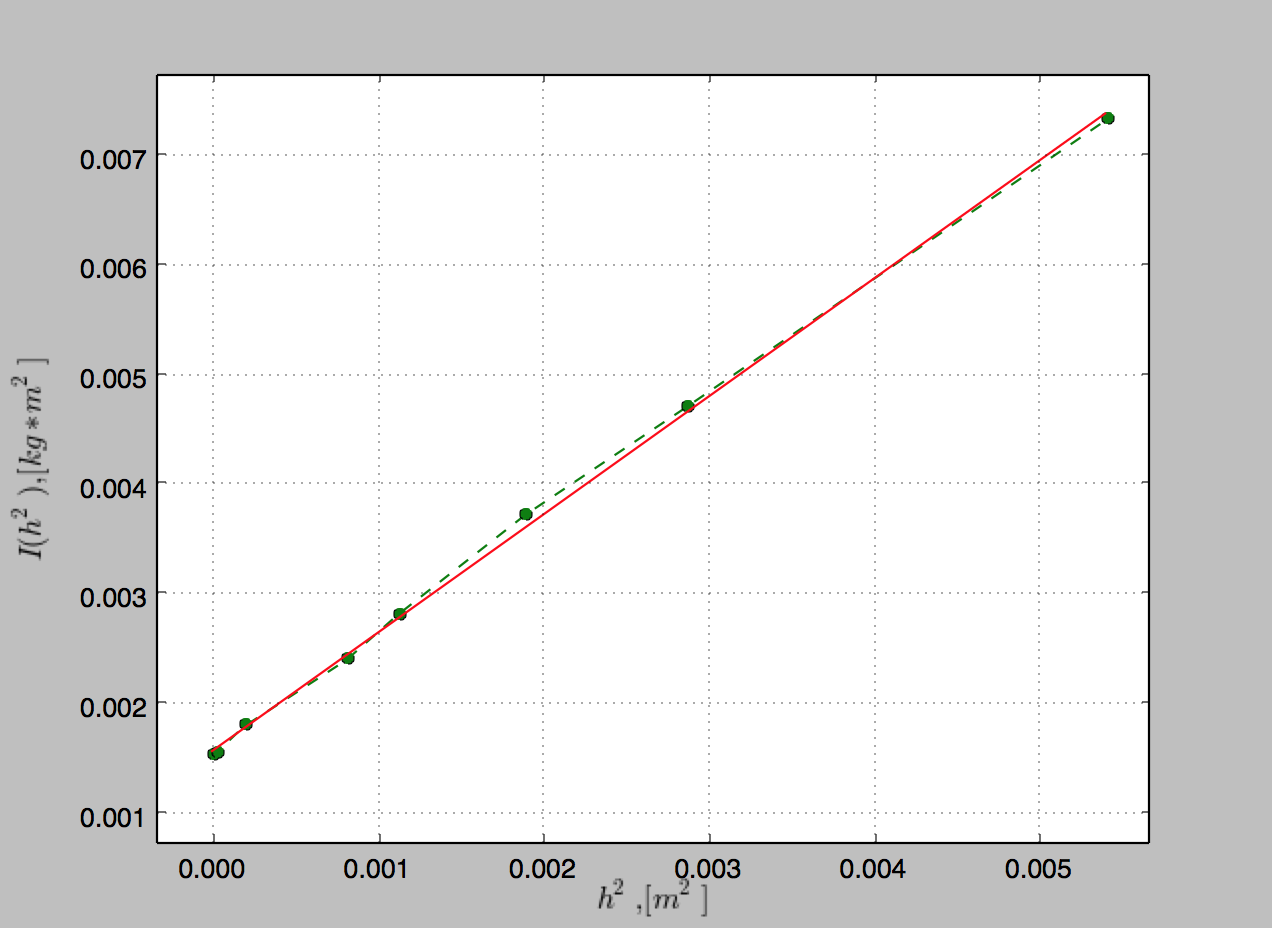
\includegraphics[width=5in]{plot.png} \\ Рис. 3: график $I(h^2)$.
            \end{center}
                $\Delta I_{max} = 0.1136 * 10^{-3} \implies I_0 = I(0) = (1.52 \pm 0.11) * 10 ^ {-3} [kg * m^2]$ \\
                Рассчитанный момент инерции диска $ I_{th} = (0.978 \pm 0.117) * 10^{-3} [kg * m^2] $ \\ 

                Коэффициент наклона прямой $k = 1.07567683217$ из закона Гюйгенса-Штейнера равен массе $m$. \\  
                $\Delta k_{max} = 0.0122017789351 \implies m = 1.0757  \pm 0.0122 [kg]$ \\
                Указанная масса диска $m_{d} = 1.1317 [kg]$.



    \end{enumerate}     
\end{document}